\chapter{Contexte et présentation}
	\section{Présentation du contexte}
	%TODO Léa : Parler du client et de son métier + besoin (cf : Cahier des charges.pdf)
		Créée en 2006, Equida est une société spécialisée dans la vente aux enchères de chevaux de course. Avec un effectif de vingt-sept personnes, la société a réalisé en 2012 un chiffre d’affaires de 87 millions d’euros. Ses clients sont des vendeurs de chevaux, principalement des haras, des entraîneurs et de grands propriétaires de chevaux, situés en France et à l’étranger. Pour être plus proche de sa clientèle étrangère, elle s’appuie sur une quinzaine de correspondants répartis dans de nombreux pays comme l’Irlande, la Turquie, ou encore le Japon.\newline
		Pour gérer son activité, la société utilise un site web qui permet notamment la consultation des ventes, une application Planning qui permet de gérer les clients, une application de gestion desventes aux enchères ainsi qu'une application de gestion des informations des chevaux.\newline
		Equida souhaite combiner ses différentes applications en une seule qui lui permettra donc de gérer les chevaux et leurs informations, leurs mises en vente, leurs enchères ainsi qu'une gestion des clients et de leur compte. Cette application combinant des fonctionnalités pour les clients (enregistrement d'un cheval, proposition d'un cheval à une vente,...) et des fonctionnalités pour l'administrateur (gestion des clients et de leur compte, validation des propositions, ajout de ventes...), elle devra contenir deux niveaux d'authentification.
		Pour plus d'informations, vous pouvez consulter la totalité du cahier des charges : \url{https://github.com/justine-martin-study/Equida/blob/master/doc/Cahier%20des%20charges.pdf}

		\noindent
		On a fait le choix de réaliser un seul projet contenant deux applications : une application web (cf: lien vers appli web) et une application mobile (cf: lien vers appli mobile) qui utilisera une api. L'application web est plus complète car destinée à être utiliser surtout par l'administrateur ; l'application mobile, elle, se concentre surtout sur des fonctionnalités propre à l'utilisateur avec tout de même quelques possibilités de gestion pour l'administrateur.

	\section{Choix techno}

		%TODO Léa : Disclamer : Pas tuto SpringBoot, gradle, ionic, ... (mettre des liens tutos)

		\subsection{MySql}
		%TODO Léa : Pourquoi avoir choisi MySql et pas autre chose
			MySql, en comparaison avec Oracle, est open source et gratuit. Ce qui le rend avantageux. \newline
			De plus, le cahier des charges fourni par le client retenait la solution de MySql pour la base de données.

		\subsection{Spring Boot}
		%TODO Léa : Pourquoi Spring boot, parler des ""parts du marchés"", avantages, ...
			On fait le choix de SpringBoot pour le projet car c'est très probablement le Framework Java pour le développement web le plus utilisé. Il permet de créer facilement un contrôleur, en effet, il suffit de créer une classe et de l’annoter @RestController. Chacune des méthodes aura l’annotation @RequestMapping qui indique quel chemin de l’API la méthode couvre et quelle méthode HTTP lui correspond.\newline
			De plus, il embarque l'équivalent d'un serveur TomCat lors de la compilation du projet (en faisant Tasks > boot > bootRun) qui permet le démarrage d'un serveur web et il s'occupe de rediriger les requêtes aux méthodes concernées. \newline
			Vous pouvez retrouver ce framework ici : \url{https://spring.io/projects/spring-boot} ainsi que des tutoriels pour l'utiliser ici \url{https://www.tutorialspoint.com/spring_boot/index.htm} et là \url{https://www.javatpoint.com/spring-boot-tutorial}

		\subsection{Ionic}
		%TODO Léa : Pourquoi Ionic, écrire du code en code Js, multiplateforme, ...
			Ionic est un framework open source qui permet de créer des applications multiplateformes (mobile et navigateur) performantes tout en utilisant des technologies Web connues (HTML, CSS, JavaScript). Il possède en plus une intégration d'Angular qui permet d'appréhender une page web comme un assemblage de composants webs indépendants mais qui peuvent communiquer entre eux. \newline
			Ionic intègre en plus des composznts visuels natifs, ainsi, les utilisateurs d'Android ou d'iOs conserveront leurs habitudes sur l'application. \newline
			Vous pouvez retrouver ce framework ici : \url{https://ionicframework.com/docs/installation/cli} avec sa documentation : \url{https://ionicframework.com/docs/components}.

		\subsection{Gradle}
			%On fait une description brève car on en reparle plus en détail dans "Intéraction entre les différentes parties du projet"
			Gradle est un "build automation system" (moteur de production). Il est un équivalent plus récent et complet à Maven. Il possède de meilleure performances, possède un bon support dans de nombreux IDE et permet d'utiliser de nombreux dépots, dont ceux de Maven.

	\section{Organisation du projet}
		\subsection{Git et branches}
			On utilise donc Git comme logiciel de gestion de versions ce qui nous permet de travailler en parallèle sur les mêmes fichiers et d'effectuer chacunes les modifications qui nous concernent sans gêner le travail de l'autre.
			\subsubsection{Branches}
			%TODO Léa : Parler de master (=version prod), develop, features/XXX
				Afin d'utiliser au mieux Git, nous avons fait le choix de créer deux branches "principales". Il s'agit donc de master et de develop.
				La branche master correspond à la version en production de nos applications. Ainsi, on ne travaillera jamais sur cette branche. Elle ne nous servira donc qu'à récupérer le contenu de la branche develop que l'on utilisera en production sur le serveur.
				La branche develop, quant à elle, est donc la branche à partir de laquelle nous travaillons. C'est à partir de cette dernière que nous créons les différentes branches pour le développement de nos fonctionnalités. Ne sont poussées sur celle-ci que les fonctionnalités opérationnels des applications. C'est donc la version en cours de développement.
				Les branches créées à partir de develop sont donc les branches correspondant aux fonctionnalités développées, elles commencent toutes par features/XXX (correspondant à la modification). Par exemple, pour la gestion des clients, on crera une branche features/gestionClients.

			\subsubsection{Nomenclature}
			%TODO Léa : Parler des nommenclatures (cf : fichier CONVENTIONS.md)
				Pour une meilleure homogénéisation de la gestion des versions, on choisit d'établir et d'utiliser une nomenclature pour les messages de commit. Cette nomenclature est consultable dans le fichier CONVENTIONS.md.
				On retrouve notamment les commits pour l'ajout de fonctionnalités sous le nom de "feat", pour les corrections de bug "fix", pour la documentation "docs", ...
				Ce qui donne des messages comme celui-ci : "feat : Ajout de la modification d'un client".


		\subsection{Les différents dossiers}
			\subsubsection{Doc}
			%TODO Léa : ((Parler de pk latex? = opensource, meilleure gestion sur git, compilation directe en pdf, ...)) + autres doc
				On a fait le choix de rédiger la documentation du projet avec Latex car c'est un système de création de documents opensource. De plus, les fichiers Latex sont facilement modifiables avec Git. On peut ainsi gérer aisément les différentes versions des documents. Il permet une compilation directe au format pdf.

			\subsubsection{SQL}
			%TODO Léa : Expliquer + nommenclature et table de version
				Les fichiers SQL (situés dans le dossier /sql) sont donc ceux qui vont créer la base de données. Il suffit d'importer les scripts dans l'ordre afin de la restituer. On nomme les fichiers précédés d'un numéro (ordre d'importation) suivi de l'intitulité de la modification. Les tables de la BDD sont en majuscules et les champs de plusieurs mots séparés d'un underscore.

			\subsubsection{Sources}
			%TODO Léa : Ionic = ionic, spring = code spring boot(webapp, rest, core) (on en reparlera plus tard dans la doc)
				Dans le dossier source, on retrouve donc deux sous-dossiers : un sous-dossier ionic et un Spring.
				Le sous-dossier ionic, comme son nom le suggère, correspond au code prore à l'application mobile (développée avec Ionic). On retrouvera à donc à l'intérieur, des fichiers json, html, service.ts. On reviendra plus en détail sur cette partie : cf lien vers le bon truc. 	%TODO Léa : FAIRE LE LIEN POV' DEBILE
				Le sous-dossier Spring, correpondant à SpringBoot, contient, quant à lui, les dossiers core, gradle, rest et webApp. Contenant notamment et respectivement les fichiers communs aux deux applications (bdd, service...), les fichiers de configuration, le code de l'api ainsi que le code de l'application web (controller, routes, formulaires, ...).
				De même, vous trouverez plus d'informations : cf lien vers le bon truc. %TODO Léa : FAIRE LE LIEN POV' DEBILE

		\subsection{Trello}
		%TODO Léa : Fournir le lien et expliquer étiquettes, Listes
			Le planning, la répartition des tâches et le fonctionnement du projet sont visibles sur le Trello : \url{https://trello.com/b/jrKixhpu/equida-spring}
			Pensez à consulter les cartes archiver pour voir le travail effectuer. En effet, les modifications effectuées sont archivées afin de ne pas les conserver dans les activités à faire.

	\section{Interactions entre les différentes parties du projet}
		\subsection{Les différentes parties}
			Le projet Équida est composé de 2 applications. Une l'application web, qui est également l'application principale, une application mobile qui est à usage principal des utilisateurs. Les 2 applications s'appuient sur la même \bdd{}. L'application web y est directement connectée. L'application mobile, elle, passe par une API. En effet, si celle ci se connecterait directement à la \bdd{} comme c'est le cas pour l'application web, une personne mal intentionnée serait en mesure de décompiler l'application mobile afin d'obtenir les identifiants de la \bdd{}. L'utilisation de cette API empêche donc notamment ce problème de sécurité.

			\begin{figure}[H]
				\centering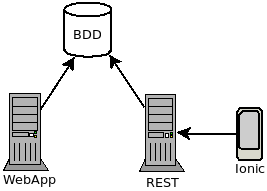
\includegraphics[width=0.45\textwidth, keepaspectratio]{res/diag_infra.png}
				\caption{La connexion à la BDD selon le projet}
			\end{figure}

			L'API ainsi que l'application web utilisent sur le Framework Spring Boot. Ces 2 applications font donc parti de 2 projets différents, "webApp" pour la partie web et "rest" pour l'api. Celles si demandant un code identique pour les Services, les Entités ainsi que les Repository, le choix a donc été fait de faire un projet commun dénommé "core" dans lequel on peut retrouver tout le code qui sera commun aux 2 autres parties, non seulement concernant les éléments cités plus haut mais également concernant les exceptions ou certains outils.

			\begin{figure}[H]
				\centering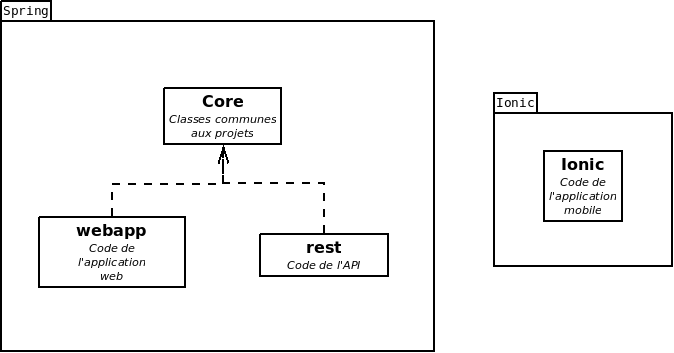
\includegraphics[width=0.75\textwidth, keepaspectratio]{res/diag_projet.png}
				\caption{Les dépendances entre les projets}
			\end{figure}

		\subsection{Configuration Gradle}

			Pour gérer correctement les différents projets basés sur Spring, leur dépendances ainsi que leur configuration nous avons donc utilisé Gradle comme mentionné plus haut. Dans le dossier "src/Spring" on retrouve le "build.gradle" qui se charge de configurer tout le projet. On peut observer la configuration suivante pour tout les projets.

			\begin{figure}[H]
				\centering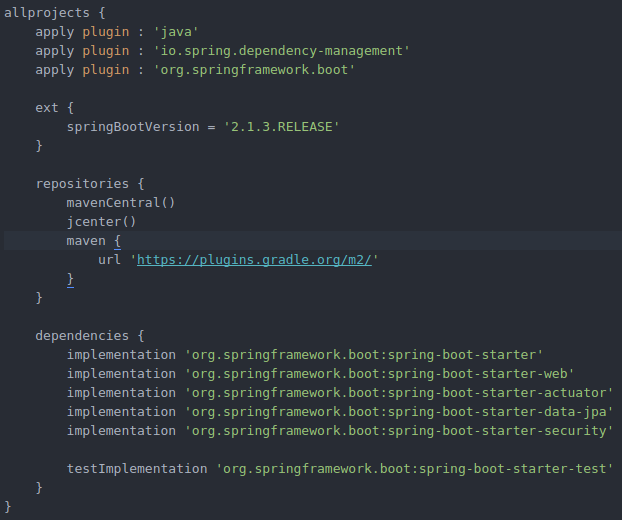
\includegraphics[width=0.75\textwidth, keepaspectratio]{res/gradle_allprojects.png}
				\caption{Configuration Gradle de tous les projets}
			\end{figure}

			On définit donc la version de Spring à utiliser, en plus des dépendences commune à chaque projet (spring-boot-starter-web, spring-boot-starter-data-jpa, ...). On va par la suite définir les dépendances uniques à chaque projet.

			\begin{figure}[H]
				\centering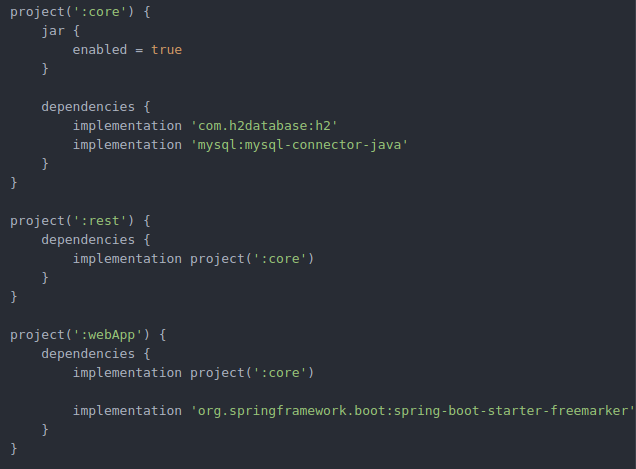
\includegraphics[width=0.75\textwidth, keepaspectratio]{res/gradle_project.png}
				\caption{Configuration Gradle individuelle des projets}
			\end{figure}

			De même, concernant le projet core, on active uniquement la compilation en jar (comme une lib) et non pas en jar bootable (comme c'est le cas lorsque l'on utilise Spring Boot).

			D'autre scripts "build.gradle" se trouvent dans chaque dossiers du projet, cependant, ceux ci ne configurent que le nom du projet à l'issue du build, la version du JDK utilisée ainsi que le package de base du projet.
